% !TeX root = ../main.tex

\chapter{绪论}

\section{研究背景及意义}

近年来,由于受到极端气候的影响,全球各地频繁发生火灾事故。例如,2021年发生在加州的山火
面积达到了9800公顷,导致2300余人被迫疏散。2019年至2020年期间,澳大利亚的山火持续了长达半
年之久,造成了巨大的生态灾难,约有30亿只动物死亡,同时也造成了不计其数的财产损失。这些火灾
不仅给人员和经济带来了巨大损失,同时还释放了大量的温室气体和有害气体,对自然环境和气候造成
了严重影响。因此,及时发现火灾、采取有效的防控措施对保护人员和国家财产的安全至关重要。

早期的火灾探测方法主要采用传统型检测设备,如感温、感烟和感光型火灾探测器等。这些设备能够在
一定程度上监测环境,并对可能出现的异常现象及时预警。然而,由于其工作原理的限制,这些传感器
往往具有灵敏度较低的缺点,并且容易受到环境影响,导致误报或漏报的情况。因此,基于图像的火灾
传感器开始被广泛应用。这些传感器通过视频监控系统和相关算法的处理分析,不仅可以精准地预警和
判断早期火灾,还可以通过实时监控图像来消除误报现象,具有极大的优势。目前常见的用于火灾探测的传感器主要有
CMOS和红外两种。CMOS传感器通过直接的视频传输进行火灾探测,而红外传感器则捕捉400到1700纳米
波段内的红外光线。然而,它们仍然存在一些问题:对于CMOS传感器,视频传输的信息量过于冗余,通
常需要提取前景才能进行后续的火灾特征提取和检测工作,同时可能出现过曝、欠曝和低对比度等问题;
而红外传感器受到其动态范围的限制,超出动态范围的高温物体如某些阳光下的物体、火焰等,均可能
表现为高灰度值的形式而难以有效区分。

为了解决这些问题,本文引入了一种新型的成像装置——事件相机,它模仿生物视网膜的原理工作\cite{gallego2020event,posch2014retinomorphic}。事件相
机与传统相机不同,它采用基于事件驱动的方式捕捉场景中的动态变化,而不是记录每一帧图像。事件相
机只记录物体的运动变化信息,如亮度变化和波长变化,通过AER协议\cite{rivas2005tools}输出模拟的生物电信号,并利用独立
的时间空间编码方式存储起来。相较于传统的RGB视频传感器,事件相机具有独特的相素独立异步工作机制,
可以有效消除冗余信息。同时,其差分成像机制和对数亮度计算可以确保较高的对比度和高动态范围内的感知。
可见,事件相机相比于前两类传统传感器更加的可靠、灵敏。

然而,基于事件相机的新颖性和前沿性,目前在火灾领域的应用尚未被充分探索,缺乏相关研究。所以,如何应用
事件相机准确而迅速地提取相关火焰特征,并基于此探索该装置在火焰检测研究工作中的可行性,是一项有重要意
义的研究课题。

\section{国内外研究现状}

\subsection{火焰成像传感器}

成像传感器的研究目前主要为可见光和红外两类。在基于可见光相机的火灾探测和识别中,通常采用数
字图像处理技术。简单来说,这一过程包括对图像进行分割、获取描述火灾图像的信息特征、检测可能
的火灾区域生长,并结合图像语义实现火灾的识别。基于可见光相机的检测具有低误报、短延迟、即时显
示现场图像、自主独立录像、现场资料保存度高等优点。目前,可见光相机在多类火灾探测上都有广泛应用。
例如,小兴安岭等类似森林区,可以利用可见光相机建立网络化监测体系,实现对林区可能火险的较及时的
监控与处理\cite{liujinxin}。再如目前矿业地区的地下作业,也在逐步投入使用类似的可见光传感器,可以对矿井火灾实现大范围、
高分辨率、高清晰度的监控,同时可见光相机的使用维护成本也较低,对矿区的环境适应性好,适合这种大规模
工作使用\cite{wyb}。

然而,在火灾探测中,可见光相机仍然面临着一些亟需解决的问题。比如,燃料的材质不同,火焰的颜色
就可能发生一些肉眼可见的变化;燃烧时的烟雾过于浓密,可见光谱图像中的火焰区域就可能被遮盖,从而导致一些
无法预见的影响。相较之下,红外相机工作原理是对火焰的红外辐射进行检测,就可以弥补可见光类传感器的上述不足。
Burnett等人\cite{burnett2018low}在工作中为红外相机添加了特殊波段的前端滤光片,从而实现了对火焰波长的高度响应。但是,红外相机
对环境的适应性就远不如可见光类传感器,常常需要使用者人工手动调整,其成本也远超可见光相机,往往要适当地
降低分辨度来大规模布局投入使用,阳光的红外等波段也对它的工作有着不小的影响。

所以,为了弥补两者的不足,本文引入了事件相机这一新型传感器,它能在自动剔除无用信息,具备低功耗优势的同时,为火焰
检测工作提供更高动态范围与采样率,期望它能够在未来的火焰检测中大放异彩,带来新机遇。

\subsection{火焰特征研究}

早期的火焰特征研究主要集中在对火焰颜色特征的提取和描述上。这些工作包括在RGB空间等\cite{chen2004early,marbach2006image,rudz2013investigation}多个不同颜色空间对各通道的火焰颜色分布
进行统计与分析。之后,有研究者基于提高火焰检测准确度的目的,逐步将一系列的火焰静态特征引入到火焰检测工作中。
如,Yamagishi等人\cite{yamagishi2000contour}的研究中,他们在HSV空间中分析火焰轮廓,利用极坐标傅里叶变换的方法,提取了波动频率。Bedo
等人\cite{bedo2015techniques}的研究中,通过MPEG-7视觉描述符,从形状、纹理等角度对相关特征进行了提取工作。此外,为了提取到更加广泛的火焰
特性,Rossi等人\cite{rossi2011use}利用双目视觉相机拍摄火焰,既可以获取纹理、边缘等此类平面性特征,还能够通过重构分析的方式,
分析一些三维信息,如火焰倾斜度和深度。同时,也有一些学者通过逐帧提取的方法,分析火焰的动态特征。例如,Chen等人\cite{2011Application}提出一种
基于火焰多种特征结合的视频火焰检测方法,采用 RGB 和 HIS 模型提取火焰候选区域k,结合火灾的动态闪烁性算法加以检测识别。
Dimitropoulos等人\cite{dimitropoulos2014spatio}在他们的工作中,综合时空特征,研究纹理的动态变化,且构建能量方程模型对燃烧加以描述。

在基于可见光相机的研究工作开展的同时,红外相机技术也在投入应用。在近红外立体视觉系统的帮助下,Rossi等人\cite{rossi2013estimation}对火点进行三维建模,
初步可实现对位置、表面、速度等几何特征的提取。秦重双\cite{qcs}对红外图像进行了滤波和形态学处理,实现对偏心度等的提取。杜志伟\cite{dzw}利用K主曲线拟合,
进行了轮廓提取工作,并基于此构建隐马尔可夫模型,预测火焰闪烁的动态过程。

\subsection{火焰数据集}

火焰数据集,往往被认为是火焰特征提取分析工作和检测识别的核心所在,目前的火焰数据集绝大部分是可见光
相机拍摄的\cite{ko2012wildfire}。常见的有:BoWFire数据集,该数据集包含了199张火焰图像和267幅正常图像,是最常用的火焰数
据集\cite{chino2015bowfire};Filckr-Fire数据集,该数据集从网络收集了5962张图片,每幅图像都由人工标注是否包含火焰,并
将存在火焰的图像分为车辆火灾、房屋火灾和森林火灾三类\cite{bedo2015techniques}。同时,为了对实时拍摄这一场景进行更加准确的模
拟,MIVIA,FurgFire这两个数据集又收集了很多真实火灾视频,这些视频大多数是使用手持设备或无人机拍摄的,
其中包含了多类的光照环境、不同的拍摄距离、大量的运动方式等,这些情况都会给检测识别工作带来新的影响与挑战。

事件相机,作为一种新型传感器,目前缺乏在火灾探测领域的应用与研究,也就更不必说
效果优良的公开数据集。所以,制作基于事件相机的火焰数据集并讨论其应用价值,是很必要的。

\subsection{火焰检测算法}

早期的学者研究工作中,主流是利用颜色特征实现对图像中火焰的检测,例如人为对颜色空间设置一个区分阈值\cite{celik2007fire}。
此外,还有一部分研究工作使用光流法、帧差法以及高斯混合模型等,以最直接的方法进行检测。但是以上两类
都共同存在低分割精度的缺陷,前者会被相似颜色物体干扰,后者会被一系列移动物体干扰。要解决这些问题,需要
基于学习的一系列方法,如Nalawade\cite{sruthiautoadaptive}利用Chan-Vese算法对全局属性进行提取(强度、区域面积等),并通过设置能
力最小方程完成了火焰和背景的分离;Tian等人\cite{tian2011smoke}在研究工作中,利用高斯混合模型和SVM对图像区域进行分类检测识别;
Toreyin等人\cite{toreyin2007online}在研究工作中构建了马尔可夫模型,以火焰的颜色运动与闪烁为参照标准实现区分。

随着深度学习方法在各个领域掀起深刻的变革,很多学者尝试将其引用到火灾探测工作中。Wang等人\cite{wang2016fire}先在RGB通道进行
初步的筛选,得到一系列可能有火焰的候选区,在训练CNN模型的基础上对其分类。张大胜等人\cite{zds}的研究中,则利用YOLO
网络,按照可能区域提取、火焰特征提取、基于提取特征进行判断的顺序进行了检测工作。按照类似的工作思路,kim\cite{kim2019video}
利用Faster R-CNN和LSTM进行了分类检测工作。基于学习的工作思路是确定的,在提取初步候选区后,间接将相关特征
参数或者直接将图像送入模型进行分类检测识别。而事件相机由于其独特的工作原理机制,排除了大量无关干扰,提取候选区
的工作被大大简化,这方面有着独特的先天优势。

\section{研究目标和内容}

本文是对事件相机在火灾探测领域应用的探索,期望达到如下目标:

1.拍摄一定规模的数据集,实现利用事件相机对火焰特征进行提取,包括静态特征和动态特征。

2.基于1中特征建立针对事件相机的较完整的火焰检测算法框架。

3.对建立的火焰检测算法的准确度与效率进行评估,探讨事件相机在火灾探测领域的可行性与应用价值。

本文采用的研究路线,如\ref{1}所示:
\begin{figure}
    \centering
    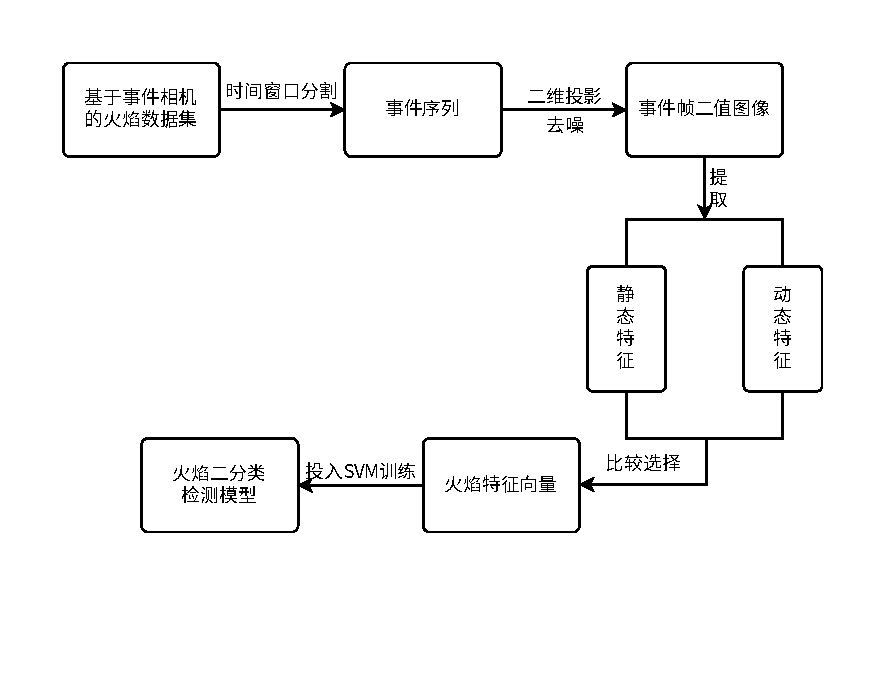
\includegraphics[width=\textwidth]{figures/thesis_flowchart.pdf}
    \caption{研究路线}
    \label{1}
\end{figure}

\section{论文章节安排}

本文内容安排如下所示:

第一章,绪论,对目前火焰检测领域的多方面研究现状进行了总结,同时介绍了引入事件相机的优势。

第二章,相关理论概述,对事件相机的基本原理以及其他相关概念作了一个较详细的阐述。

第三章,基于事件相机的数据集构建,对火焰数据集的拍摄构建过程进行了较详细的介绍。

第四章,基于事件相机的火焰特征提取,详细介绍了如何从事件数据中还原火焰区域并提取常用的火焰静态和动态特征,
构建提取算法框架,同时也对其中的一些特征进行了初步分析。

第五章,基于事件相机的火焰检测算法,详细介绍了如何利用支持向量机构建火焰检测算法框架,以及对算法准确度和效率进行客观指标评估等内容。

第六章,工作总结与展望,对实验结果与创新点进行总结,同时对其中的缺陷不足提出未来的改进展望。
